\section{INFORME PREVIO}

\begin{enumerate}[label=\alph*)]
    \item Analizar y Diseñar un oscilador con un NE555 de 10KHz.\\
    En el modo astable, el temporizador 555 forma una salida continua de señal rectangular con una frecuencia específica que tiene posiciones fijas de la señal de salida en un estado alto y bajo con dos resistencias y un capacitor. Cuando el temporizador 555 en el modo astable recibe energía por primera vez, el capacitor comienza a cargar con voltaje, lo que lleva a una señal de salida alta. Mientras el capacitor se carga hasta llegar a 2/3 del voltaje de suministro del IC. En ese punto, el capacitor comienza a descargarse, lo que lleva a una señal de salida baja. Cuando el voltaje en el capacitor desciende a 1/3 del voltaje de suministro del IC, comienza a cargar nuevamente, lo que lleva a una señal de salida alta y el proceso se repite.\cite{NE555}
    \begin{figure}[H]
        \centering
        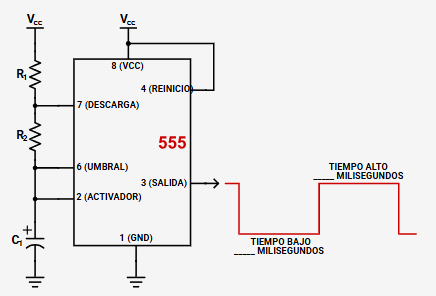
\includegraphics[width=.7\textwidth]{imgs/3.1. 555 Esquemático.png}
        \caption{Esquemático de un oscilado 555 astable}
    \end{figure}
    El comportamiento de un oscilador astable NE555 se describe con las siguientes fórmulas
    \begin{align*}
        T_h&=0.693(R_1+R_2)C_1\\
        T_l&=0.693R_2C_1\\
        f&=\frac{1.44}{(R_1+2R_2)C_1}
    \end{align*}
    Para tener un ciclo de trabajo del 50\%, se selecciona un $R_2$ bastante grande para que $R_1$ haga mucha diferencia entre los tiempos alto y bajos. Para eso, $R_2$ lo seleccionamos como $1M\Omega$. Para que $T_L$ sea cercano $50\mu s$ (para una frecuencia de $10kHz$), se selecciona un capacitor comercial de $68pF$. En consecuencia, $R_1$ podría tomar valores comerciales menores a $5k\Omega$ para mantener una relación cercana al 50\%. Por ejemplo, con $R_1=4.7k\Omega$.
    \begin{align*}
        f = \frac{1.44}{(4.7k+2M)6.8p} = 10.56kHz.
    \end{align*}
    \newpage
    \item Explicar brevemente los tipos de filtros que se usan en un PLL, señalando las ventajas y desventajas de su uso.\\
    Los filtros que acompañan el detector de fase de un PLL son todos pasabajos. Su función es ajustar la respuesta del PLL, haciéndola más rápida o más estable. Cuando el detector de fase es ideal, el filtro no es necesario.
    
    Cuando el comparador de fase no es ideal el filtro pasa a ser necesario. El caso más simple es cuando se trata de un sencillo pasabajos RC, cuya FT es\cite{PLL}:
    \begin{figure}[H]
        \centering
        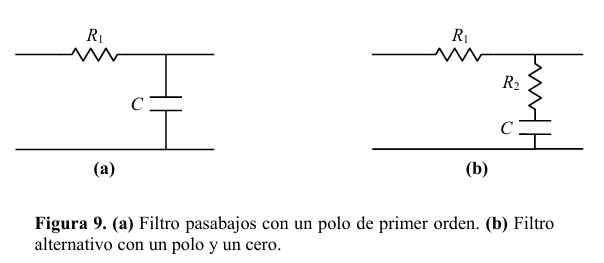
\includegraphics[width=.7\textwidth]{imgs/3.2. PLL Filtros.png}
        \caption{Filtros pasabajos de primer orden\cite{PLL}}
    \end{figure}
    \begin{align*}
        F_1(s)=\frac{1}{1+RCs}
    \end{align*}
    Lo que al introducirse en la función de transferencia del PLL, genera:
    \begin{align*}
        \frac{V_0(s)}{\Omega_i(s)} = \frac{1}{K_{OSC}}\frac{1}{1 + \frac{1}{K_{OSC}K_DA}s + \frac{RC}{K_{OSC}K_DA}s^2}
    \end{align*}
    Lo que da una función de transferencia de segundo orden, con valores característicos:
    \begin{align*}
        \omega_n &= \sqrt{\omega_{RC}K_{OSC}K_DA}\\
        \xi &= \frac{1}{2}\sqrt{\frac{\omega_{RC}}{K_{OSC}K_DA}}
    \end{align*}
    Debe tenerse en cuenta que $\omega_{RC}$ debe ser relativamente pequeño, para poder filtrar la frecuencia $\omega_i + \omega_{VCO} \cong 2\omega_i$. Al mismo tiempo, como $\omega_n$ determina el ancho de banda resultante para el PLL, debe adoptarse lo suficientemente grande para permitir el paso de la máxima frecuencia de variación de la frecuencia de entrada. Esto en general impone limitaciones que se traducen en  bajos valores de $\xi$. La consecuencia será un sistema con una respuesta muy subamortiguada, lo cual no es deseable.

    En caso se tenga un filtro con un polo y un cero, la función de transferencia del filtro sería:
    \begin{align*}
        F_2(s)=\frac{1+R_2Cs}{1+(R_1+R_2)Cs}
    \end{align*}
    Cuyos valores característicos serían:
    \begin{align*}
        \omega_{PLL} \cong \omega_n &= \sqrt{\omega_1K_{OSC}K_DA}\\
        \xi &= \frac{1}{2} \omega_n \left( \frac{\omega_{RC}}{K_{OSC}K_DA} + \frac{1}{\omega_2}\right)
    \end{align*}
    \begin{figure}[H]
        \centering
        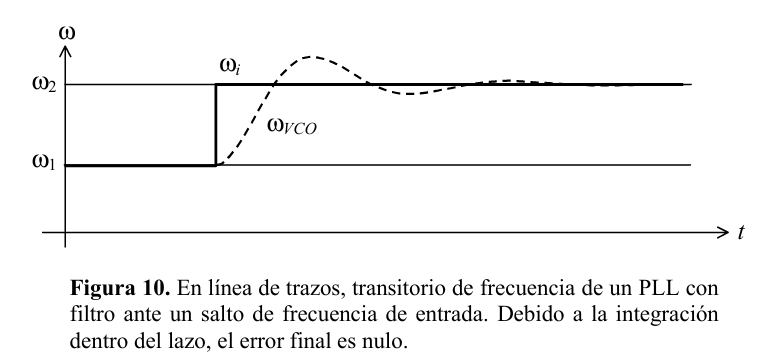
\includegraphics[width=.7\textwidth]{imgs/3.2. Respuesta a un escalón.png}
        \caption{Transitorio de un PLL con un filtro de segundo orden}
    \end{figure}    
    \item Diseñar el filtro más conveniente para este caso.
    \begin{figure}[H]
        \centering
        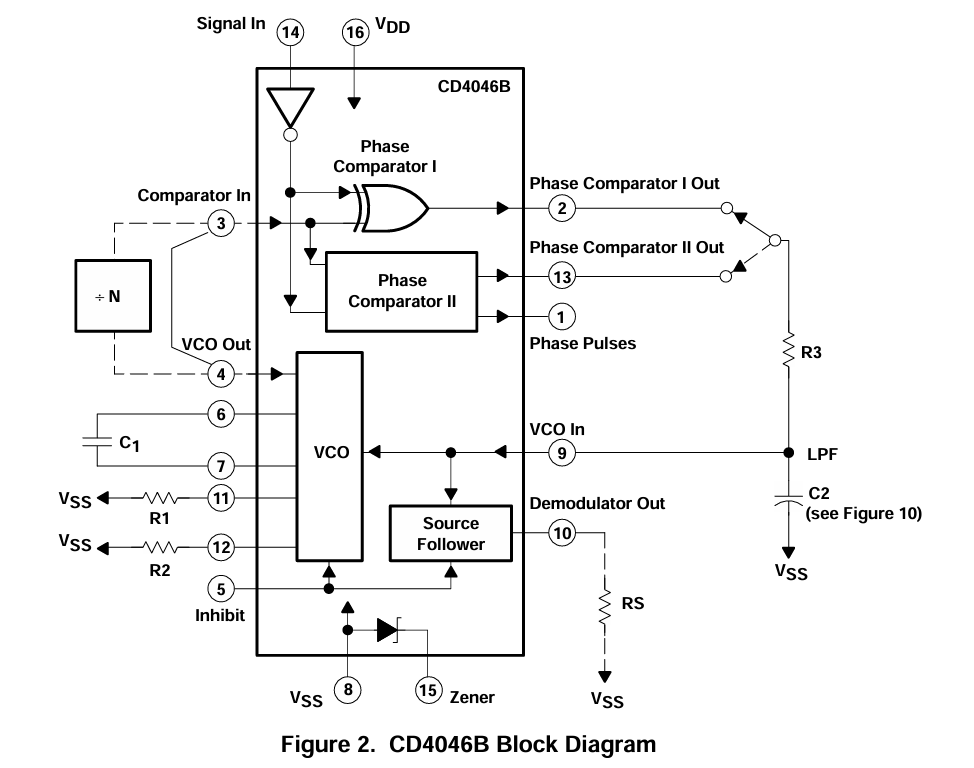
\includegraphics[width=.6\textwidth]{imgs/3.3. Diagrama de bloques del 4046.png}
        \caption{Diagrama de bloques del 4046}
    \end{figure}
    Para el filtro pasabajos (LPF) entre los pines 2/13 y 9, se tomó en cuenta el que PLL 4046 fue diseñado para tener un rango de captura de (según datasheet):
    \begin{align}
        f_c \approx \pm \left( \frac{1}{2\pi} \right) \left( \frac{2\pi f1}{R_3C_2} \right) = \pm 0.4kHz
    \end{align}
    Para la aplicación se eligió un filtro con cero y un polo, de forma que $R_3$ es $27k\Omega$, y en la rama de $C_2$, se coloca un resistor en serie de $330\Omega$ y se elige un $C_2$ de $4.7\mu\Omega$
    \item Explicar brevemente la función de los divisores de frecuencia y las posibilidades de división de un 7493 y un PIC16f628A.
    \begin{figure}[H]
        \centering
        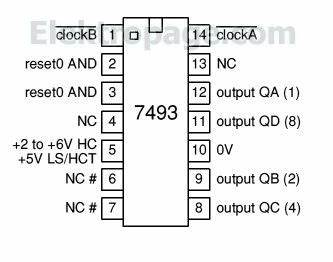
\includegraphics[width=.5\textwidth]{imgs/3.4. 7493 pinout.jpg}
        \caption{7493 pinout}
    \end{figure}
    Teniendo como entrada clockA, y conectando la entrada clockB a la salida output QA, se puede tener 4 salidas:
    \begin{itemize}
        \item Divisor por 1: QA (pin 12)
        \item Divisor por 2: QB (pin 9)
        \item Divisor por 4: QC (pin 8)
        \item Divisor por 8: QD (pin 11)
    \end{itemize}
    \begin{figure}[H]
        \centering
        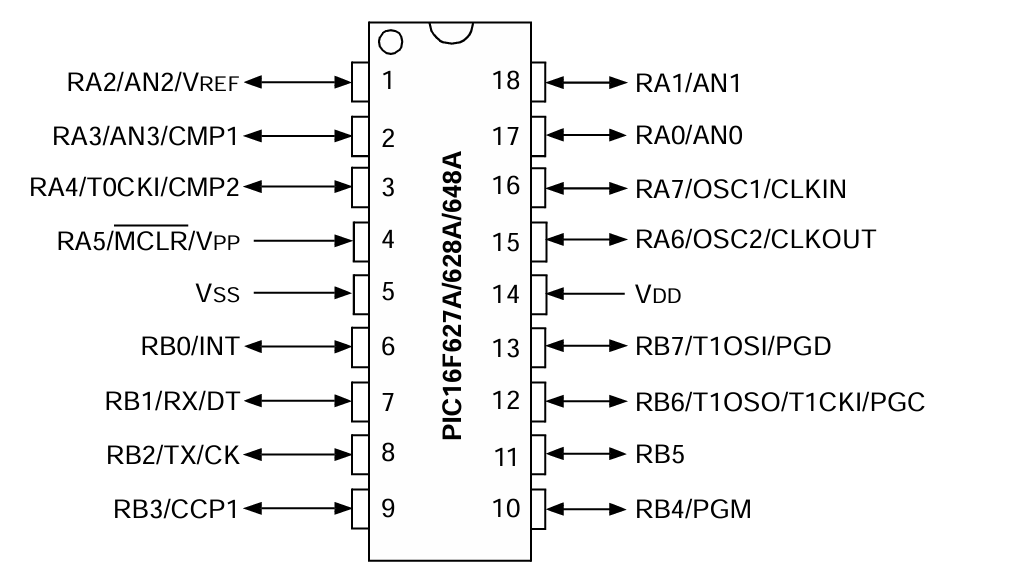
\includegraphics[width=.5\textwidth]{imgs/3.4. 16F628A pinout.png}
        \caption{16F628A pinout}
    \end{figure}
    De los 16 pines I/O digitales, repartidos en los registros A y B, del PIC16f628A, un acercamiento sencillo para la división de frecuencia sería contar la cantidad de flancos en un pin de entrada y después de un número determinado de ellos se genere un flanco, o cambio de estado, en otro pin de salida. Para permitir una división de frecuencia ajustable por el usuario, se pude cnfigurar que los pines de entrada/salida del divisor se encuentren en un solo registro  (por ejemplo, el A) y el otro registro por completo sea utilizado para determinar la cantidad de flancos que se deben contar antes de cambiar el estado del pin de salida, a modo de referencia.
    \item Utilizar un simulador para observar el comportamiento de los circuitos diseñados y propuestos
    \begin{figure}[H]
        \centering
        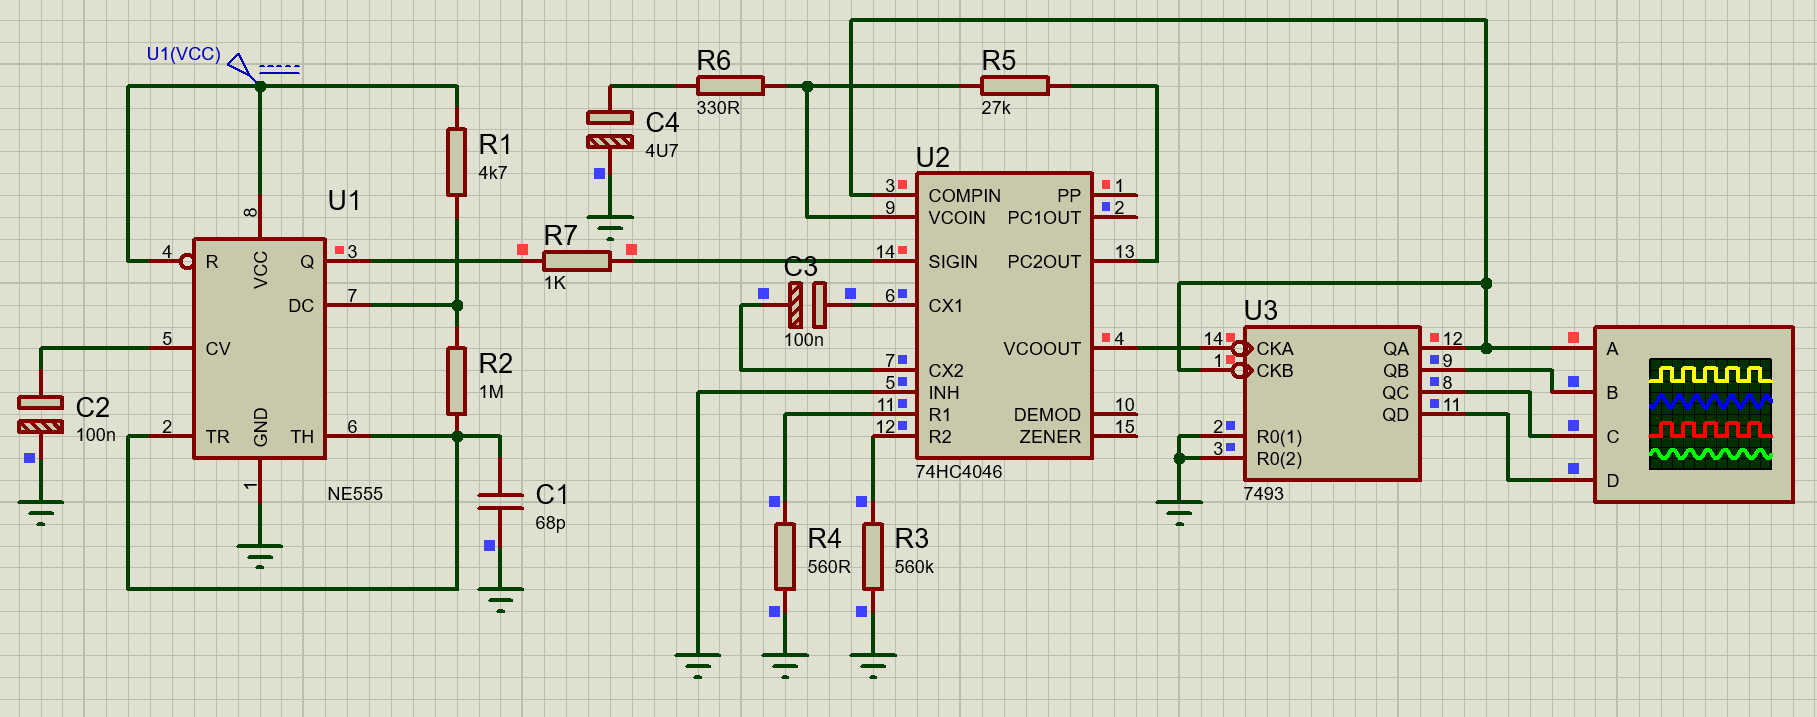
\includegraphics[width=.9\textwidth]{imgs/3.5. Esquemático.png}
        \caption{Simulación utilizando un 7493}
    \end{figure}
    {\it Nota: El resistor R7 fue colocado para evitar errores de convergencia en la simulación, no es necesario en una aplicación real.}
    \begin{figure}[H]
        \centering
        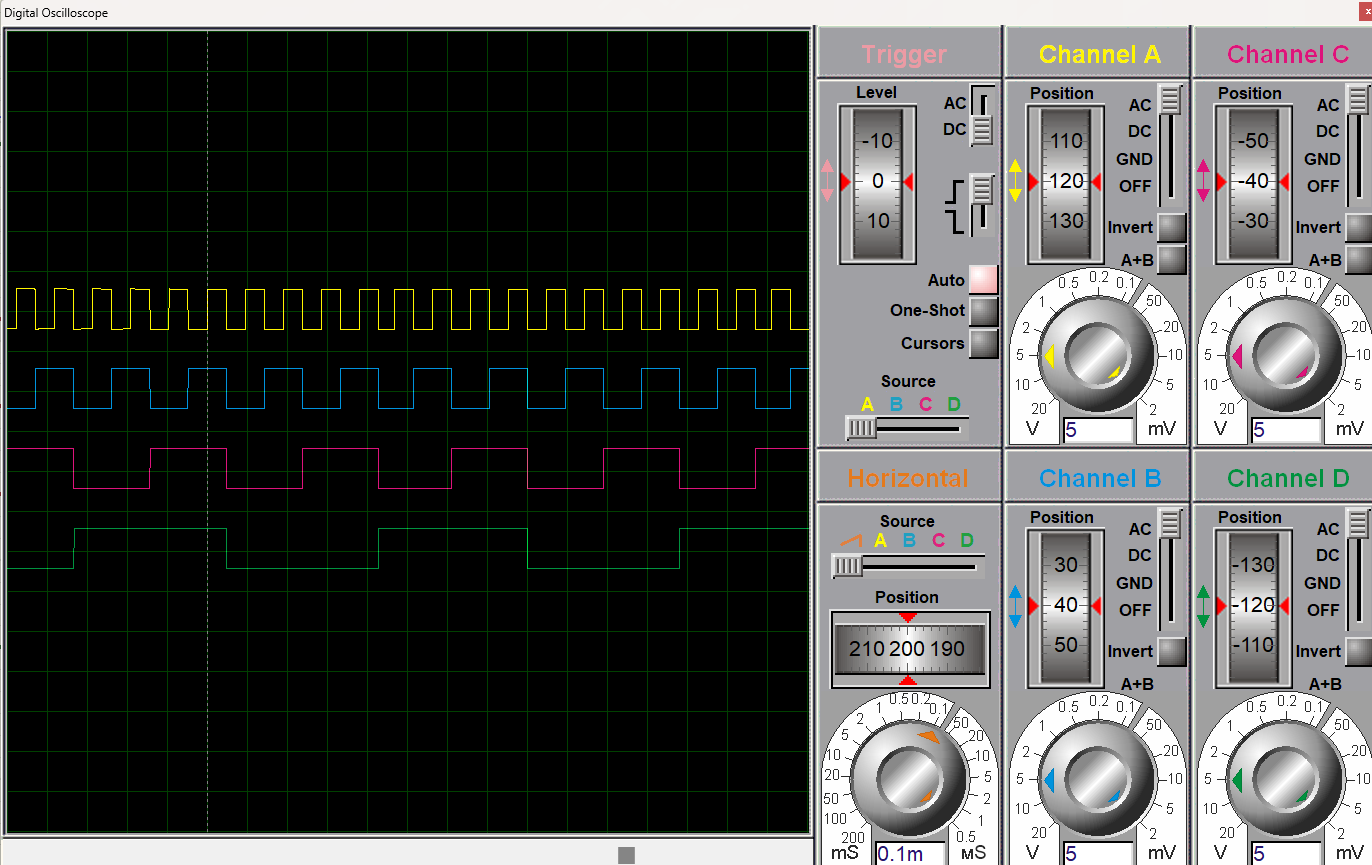
\includegraphics[width=.9\textwidth]{imgs/3.5. Osciloscopio.png}
        \caption{Osciloscopio simulado}
    \end{figure}
    Como se ve, el 7493 permite la división de la señal de entrada con los factores de x1, x, x4 y x8 las cuáles se pueden elegir para ser retroalimentadas al comparador de fase y conseguir el mismo factor pro de multiplicación para la salida del VCO. Si se desease otro valor operando los 4 bits de salida, se requeriría un circuito lógico de control adicional.
    \begin{figure}[H]
        \centering
        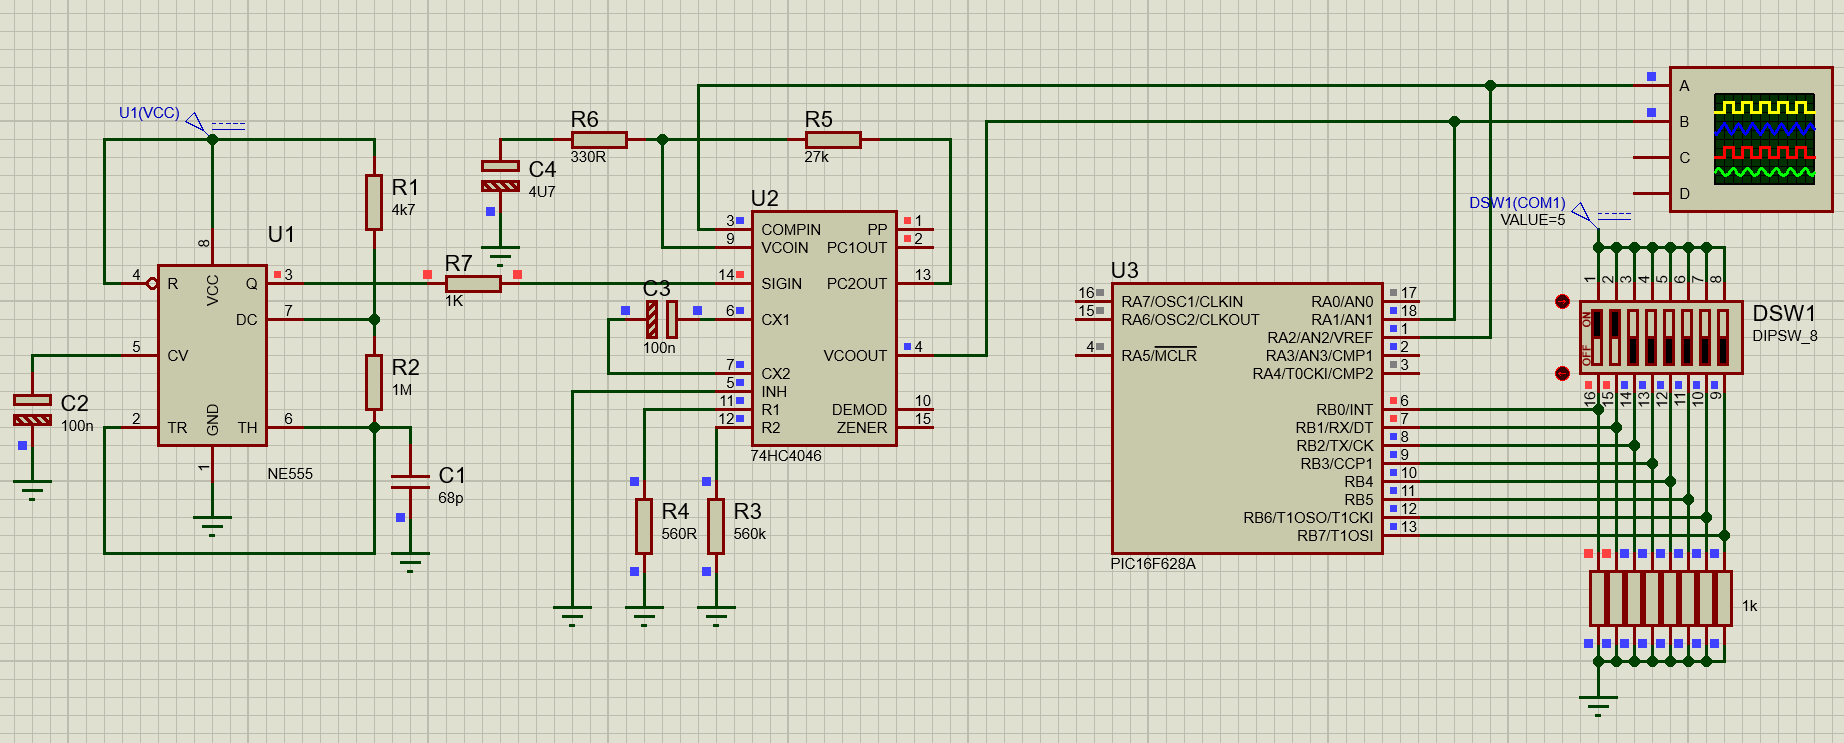
\includegraphics[width=.9\textwidth]{imgs/3.5. Simulación con PIC.png}
        \caption{Divisor de frecuencia usando un PIC16F628A16F628A}
    \end{figure}
    {\it Nota: El resistor R7 fue colocado para evitar errores de convergencia en la simulación, no es necesario en una aplicación real.}
\end{enumerate}